\chapter{Architecture design} \label{ch:archdesign}
\todo{NOT DONE! rough sketch. De nedenstående trin er hvad jeg skal igennem: Para. Anal., Alloc., Optimizaiton, FSMD og VHDL + simulering }
This chapter will describe the design process for the hardware architecture. In section \ref{sec:ParaAnal} a parallelism analysis is performed. Section \ref{sec:AllocSched} will describe the allocation and scheduling of the hardware elements.

\section{Parallelism Analysis}\label{sec:paraanal}
The inherent parallelism of the system has been analyzed to find out which improvements can be made. Figure xx shows a diagram of the whole system and on the following pages, data flow graphs (DFG) for each subsystem can be found. \\

\begin{figure}[ht!]
  \centering
  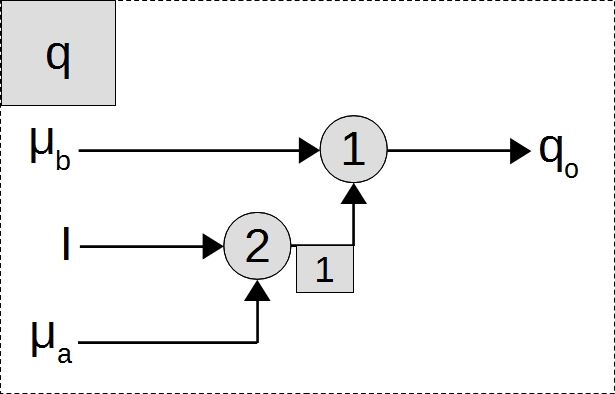
\includegraphics[scale=0.3]{figures/SDFG_q}
  \caption{Synchronous data flow graph of the q block in the guided image filter}
  \label{fig:sdfg_q}
\end{figure}

To find the parallelism in the system precedence graphs (PG) have to be created. Since the subsystems are simple the precedence graphs can be created looking at the system from end to start and for each operator find out which signal is needed and have to be calculated before. Another method is to create a synchronous data flow graph (SDFG) and from the SDFG a matrix, $\uuline\Gamma$, can be created. This matrice expresses the relationship between the in- and outputs from each node in the SDFG and is called the \textit{topology} matrix. An example of an SDFG is illustrated on in figure \ref{fig:sdfg_q}. In this example the topology matrix is then:
\begin{equation}
  \begin{array}{ c c c }
    & & \text{nodes} \\
  \uuline\Gamma = & \text{arcs} & 
  \begin{bmatrix}
   -1 & 1 
  \end{bmatrix}
  \end{array}
\end{equation}
If $rank(\uuline \Gamma) \leq s-1$ where $s$ is the number of nodes then a positive integer vector $\uline q$ can be found such that $\uuline\Gamma \cdot \uline q = \uline 0$. Then resulting $\uline q$ is:
\begin{equation}
  \uline{q} =
  \begin{bmatrix}
  1 \\
  1
  \end{bmatrix}
\end{equation}
This $\uline q$ vector expresses how many times each node have to be executed within one sample period.\\

With $\uuline \Gamma$ and $\uline q$ a periodic admissible sequential sequence (PASS) can be found. This tells a sequential sequence in which the nodes can be executed and with it, a periodic admissible parallel sequence (PAPS) can be generated. To find the PASS generate a randomly ordered list of all the nodes, $L$. For each 

\section{Allocation and Scheduling}\label{sec:allocsched}
To develop a Finite State Machine (FSM) we need to know which hardware is allocated and when each operation is scheduled. This enables us to define some states for the FSM.

From section~\vref{sec:paraanal} some precedence graphs are found and theses graphs shows how many FUs can run in parallel. We need to know how much hardware is needed for each FU. To calculated some simple system have been generate in Vivado 2016.2 and then synthesized. Then utilization of the hardware can be found. Appendix~\vref{app:alloctest} describes in detail the procedure and table~\ref{tab:utilizationofelements} shows the result.
\begin{table}[ht!]
\centering
\begin{tabular}{l | c c c c }
  \toprule
   &  LUT & FF & BRAM & DSP48 \\
  \midrule
  Adder & 15 & 15 & - & - \\
  Adder/Subtracter  & $\approx 16$ &  15 & - & - \\
  Subtract  & 15 &  15 & - & - \\
  Multiplier - LUT  & 352 &  36 & - & - \\
  Multiplier - DSP48 & - & - & - & 1 \\
  Divider & $\approx 177$ & 82 & 0.5 & 7 \\
  \bottomrule
\end{tabular}
\caption{Number of logic elements used in average for each FU}
\label{tab:apputilizationofelements}
\end{table}

To create the FSM specification we need to introduce time into the precedence graphs to establish some states. To achieve this scheduling is used. There exists different methods for scheduling and some of these are:
\begin{itemize}
  \item Resource Constrained (RC)
  \item Time Constrained (TC)
\end{itemize}

\subsection{RC scheduling}
\todo{lav om til operation og husk mult}
For both methods the first step is create as soon as possible (ASAP) and as late as possible (ALAP) schedules. Then for the RC scheduling a ready list is created. This list contains a list of operations which are ready for scheduling and sorted by mobility. The mobility, $M(op)$, expresses the difference between the states in which the operation, $op$, have been scheduled in ASAP and ALAP schudules, e.i. $S_{ALAP}(op) - S_{ASAP}(op)$. \\
Figure \vref{fig:sch_asap_alap} shows an example of an ASAP and an ALAP schedule. As seen on the figure node 1-10, 13, 17, 20 and 22-23 are part of the critical path and therefore mobility is 0 for each of the nodes. Nodes 11-12,14-15,18 and 21 all have a mobility of 2 and nodes 16 and 19 have a mobility of 3. \\
\begin{figure}[ht]
  \centering
  \begin{subfigure}[t]{0.45\textwidth}
    \centering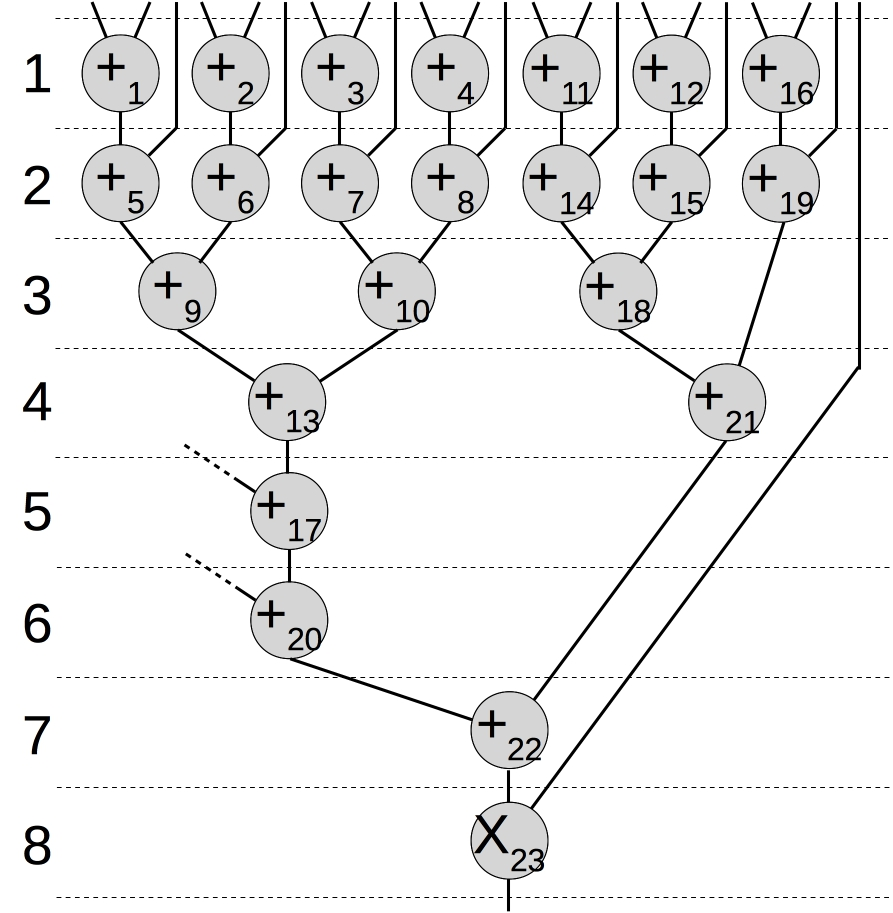
\includegraphics[height=6.5cm]{figures/sch_mfilt_asap.jpg}
    \caption{Example of ASAP schedule\label{fig:sch_asap}}
  \end{subfigure}\hspace{0.5cm}
  \begin{subfigure}[t]{0.45\textwidth}
    \centering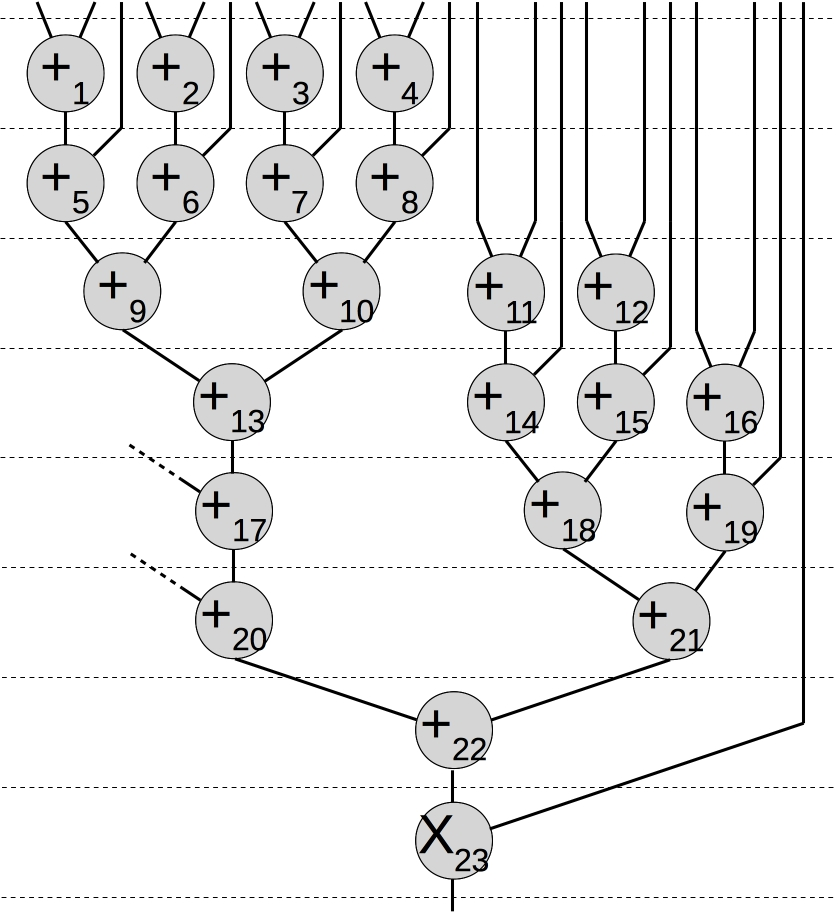
\includegraphics[height=6.5cm]{figures/sch_mfilt_alap.jpg}
    \caption{Example of ALAP schedule\label{fig:sch_alap}}
  \end{subfigure}
  \caption{Illustration of ASAP and ALAP schedules. The illustration shows a part of the mean filter shown on figure~\vref{fig:bla} \label{fig:sch_asap_alap}}
\end{figure}

With mobility found for each node/operation then a ready list can be generated. Add every ready node and then sort them by mobility. In the start the list would look like this: 1. node 1 ($M(+_1)=0$), 2. node 2 ($M(+_2)=0$), 3. node 3 ($M(+_3)=0$), 4. node 4 ($M(+_4)=0$), 5. node 11 ($M(+_{11})=2$), 6. node 12 ($M(+_{12})=2$) and 7. node 16 ($M(+_{16})=3$).\\

Lets say the system have 3 ALU's available then node 1-3 can be scheduled to state 1 since they are higher on the ready list and there is no free ALU for the remaining nodes. The scheduled nodes are removed and the ready list is updated with newly available nodes. The list is still sorted by mobility and will now look like this: 1. node 4 ($M(+_4)=0$), 2. node 5 ($M(+_5)=0$), 3. node 6 ($M(+_6)=0$), 4. node 7 ($M(+_7)=0$), 5. node 11 ($M(+_{11})=2$), 6. node 12 ($M(+_{12})=2$) and 7. node 16 ($M(+_{16})=3$). \\

Then nodes 4-6 are scheduled into state 2 since they have lower mobility than the rest of the ready list. The list is updated again and will look like this: 1. node 7 ($M(+_7)=0$), 2. node 8 ($M(+_8)=0$), 3. node 9 ($M(+_9)=0$), 4. node 11 ($M(+_{11})=2$), 5. node 12 ($M(+_{12})=2$) and 6. node 16 ($M(+_{16})=3$).\\

Nodes 7-9 are scheduled into state 3 and the list is updated again: 1. node 10 ($M(+_10)=0$), 2. node 11 ($M(+_{11})=2$), 3. node 12 ($M(+_{12})=2$) and 4. node 16 ($M(+_{16})=3$).\\
\begin{figure}[ht!]
  \centering
  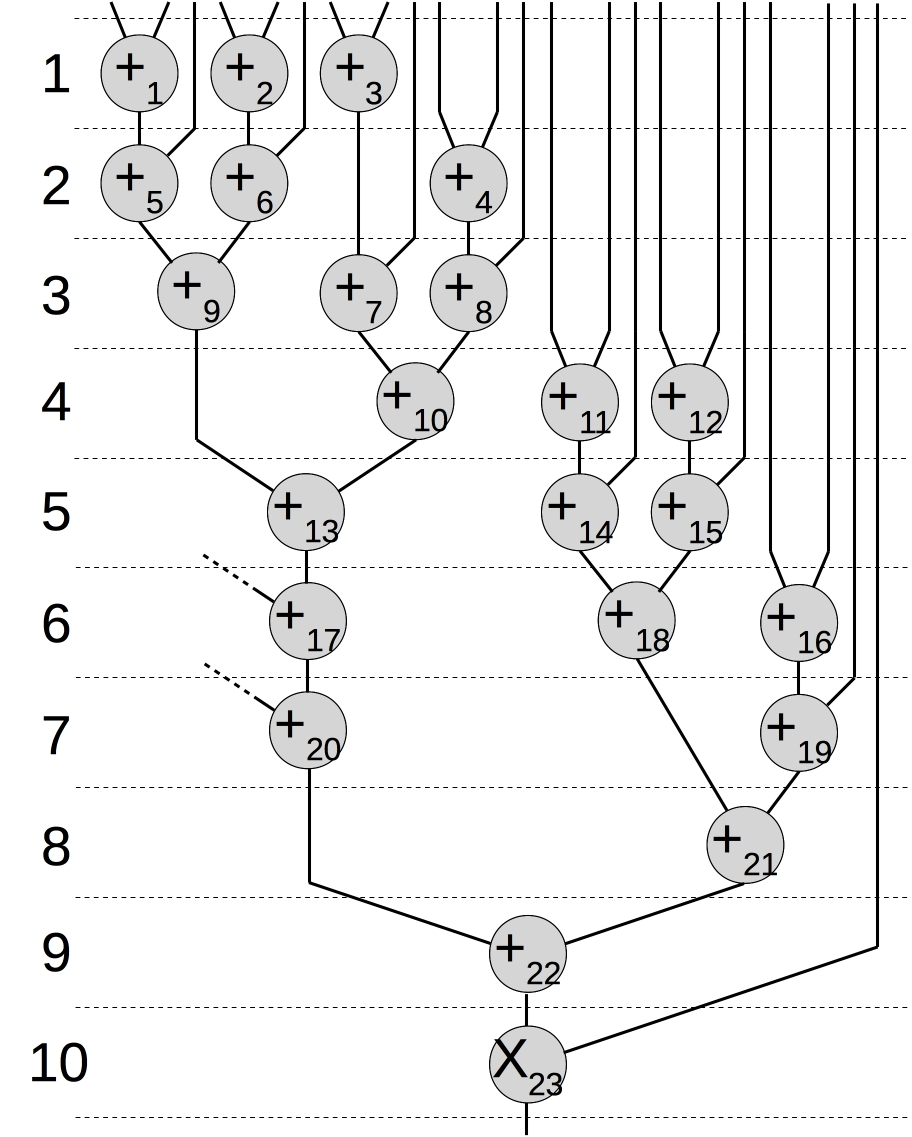
\includegraphics[height=8.125cm]{figures/pc3alu.jpg}
  \caption{RC schedule}
  \label{fig:rc3alu}
\end{figure}

This is repeated until all nodes have been scheduled and the result is seen in figure \vref{fig:rc3alu}. This schedule uses 2 states more than the ASAP and ALAP but it reduces the cost since it uses 1 less ALU than the ALAP schedule and 5 less than the ASAP schedule.  \\
This information is described in \cite{gajski2009}.

\subsection{TC schedule}
The RC schedule improves the cost of the \todo{find et bedre ord}implementation while the TC intends to improve the performance of the implementation. First a maximum number of states is decided and then ASAP and ALAP schedules are generated and mobility ranges are found. Then some probabilities are assigned to each operation. These probabilities express the probability for the specified operation to be scheduled in each state in its mobility range e.g. operation 11 in \vref{fig:sch_asap_alap} have $1/3$ probability for being scheduled in each of state 1-3 if maximum number of states is kept at 8. Figure \vref{fig:tc_prob} shows the probabilities for each operation in figure \vref{fig:sch_asap_alap}.
\begin{figure}[ht!]
  \centering
  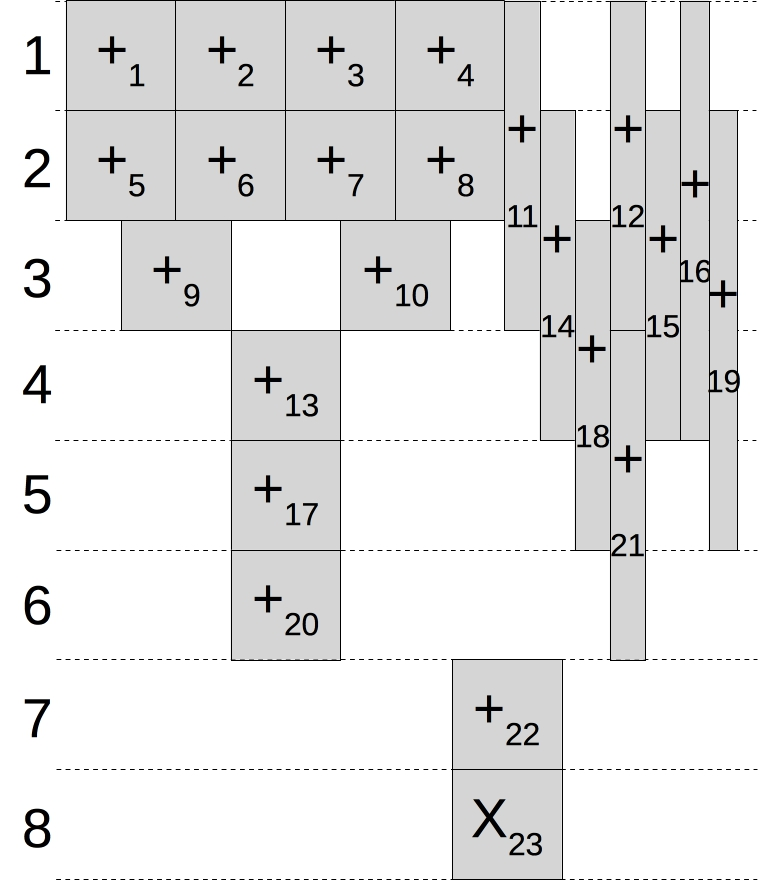
\includegraphics[height=6.5cm]{figures/tcscheprob}
  \caption{Probabilities for each operation in figure \vref{fig:sch_asap_alap}}
  \label{fig:tc_prob}
\end{figure}
{\color{gray}Fortsæt med at skrive senere}


\section{Finite State Machine with Data Path design}
\subsection{FSMD example}
This section will contain an example of a FSMD design example but only of a small part of the system to show have to design a FSMD but also to show that it is a really extensive process. For this example the $b$ block (see figure \vref{fig:b_par}) from the guided image filter (see figure \vref{fig:Guided_image_filter}) and it is shown here on figure \vref{fig:b_FSMD_1}.
\todo{tjek op på synkront dataflow diagram og state diagram}
\begin{figure}[ht]
  \centering
  \begin{subfigure}[t]{0.45\textwidth}
    \centering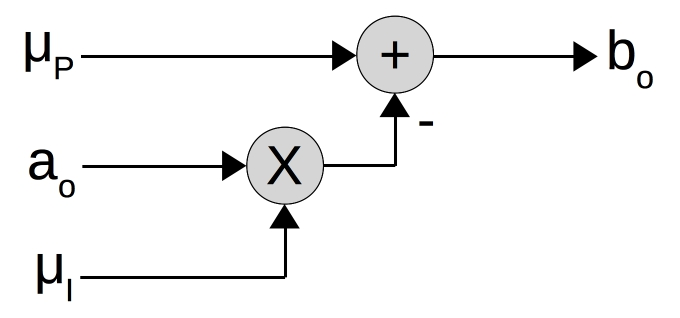
\includegraphics[scale=0.4]{figures/b_FSMD_1}
    \caption{$b$ block\label{fig:b_FSMD_1}}
  \end{subfigure}\hspace{0.5cm}
  \begin{subfigure}[t]{0.45\textwidth}
    \centering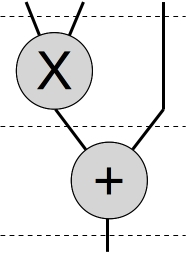
\includegraphics[scale=0.4]{figures/b_FSMD_SSD}
    \caption{Synchronous State Diagram of the $b$ block\label{fig:b_FSMD_SSD}}
  \end{subfigure}
  \caption{$b$ block FSMD stuff\label{fig:b_FSMD_1_all}}
\end{figure}

\begin{figure}[ht!]
  \centering
  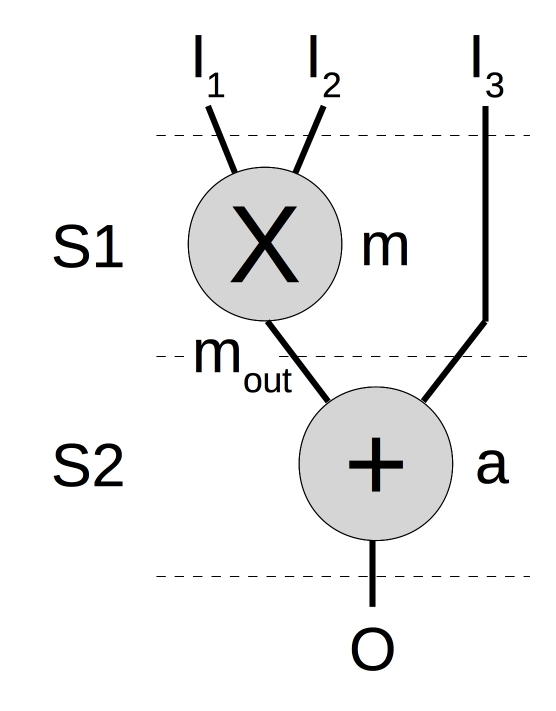
\includegraphics[scale=0.225]{figures/b_FSMD_SSD_extended}
  \caption{Synchronous State Diagram with every connection, functional units, in- and outputs named}
  \label{fig:b_FSMD_SSD_ext}
\end{figure}


\begin{table}[ht!]
  \centering
  \begin{tabular}{r | c | c}
  \toprule
  & S$_1$ & S$_2$\\
  \midrule
  I$_1$ & $\surd$ & \\
  I$_2$ & $\surd$ & \\
  I$_3$ & & $\surd$ \\
  m$_{\text{out}}$ & & $\surd$ \\
  O & & $\surd$
  \end{tabular}
  \caption{Life-time analysis}
  \label{tab:b_FSMD_lifetime_anal}
\end{table}

\begin{figure}[ht!]
  \centering
  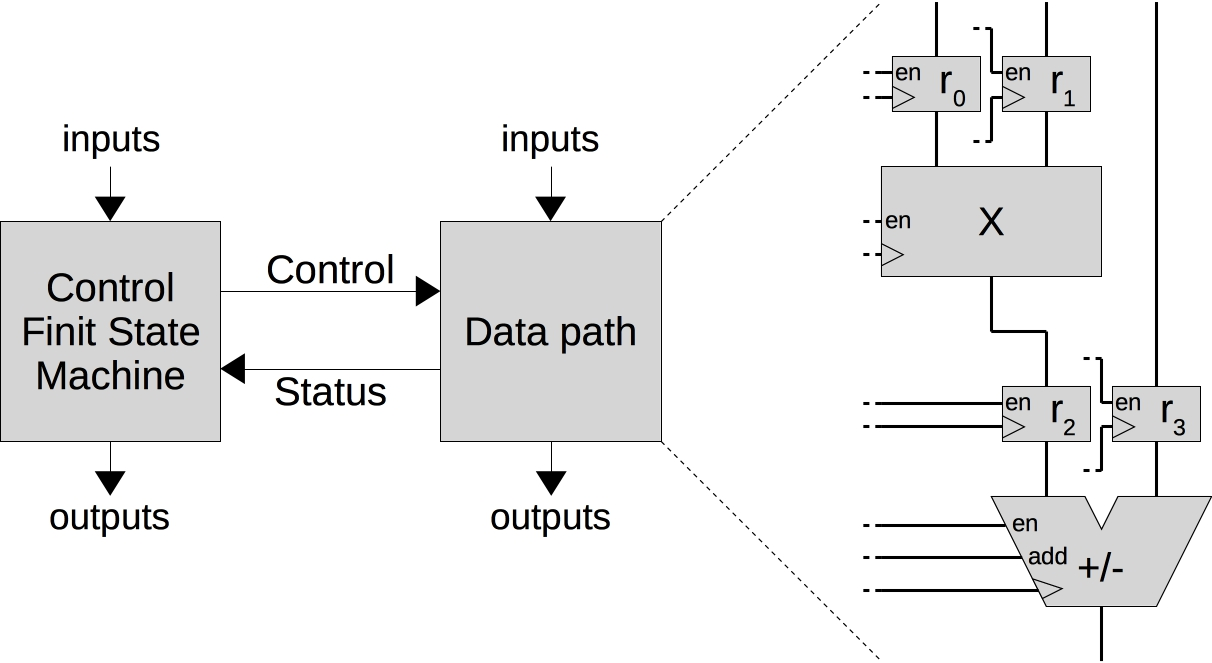
\includegraphics[scale=0.3]{figures/b_FSMD_full}
  \caption{Finite State Machine with Data path and the design of the data path is shown.}
  \label{fig:b_FSMD_full}
\end{figure}
\todo{tænk i register! transfer! level og ikke i FSMD}
\begin{lstlisting}
-- test
...
begin
  process (clk)  -- Sequential process
  begin 
    if rising_edge(clk) then
      state <= next_state;
    end if;
  end process;
  
  process (state, reset, cars, short, long)  -- Combinational process
  begin
    if reset = '1' then
      next_state <= S1;
    else
      case state is
        when S1 =>
          m_out = I_1 * I_2;
        when S2 =>
          r_2 <= m_out;
          O <= r_2-I_3;
      end case;
    end if;
  end process;      
\end{lstlisting}

\color{gray}
\section*{noter til mig selv}
% ---------------------- udkommentere senere --------****
Controller <--signaler--> Data path\\
Controller:\\
Data path:  indeholder register, FU, connections, network osv.

skal jeg lave et eksempel med en lille del af mit system? så kan man se hvor voldsomt det kan blive og se processen. Derefter kan jeg vise hvad jeg kommer frem til

noter fra møde med peter:\\
- lifetime analysis \\
- synchronous diagram
\color{black}

\newpage
% precedence graphs --------------------------------------------------------------------------------------------------- --------------------------------------------------------------------------------------------------- --------------------------------------------------------------------------------------------------- --------------------------------------------------------------------------------------------------- --------------------------------------------------------------------------------------------------- --------------------------------------------------------------------------------------------------- --------------------------------------------------------------------------------------------------- --------------------------------------------------------------------------------------------------- 
\begin{figure}[ht!]
  \centering
  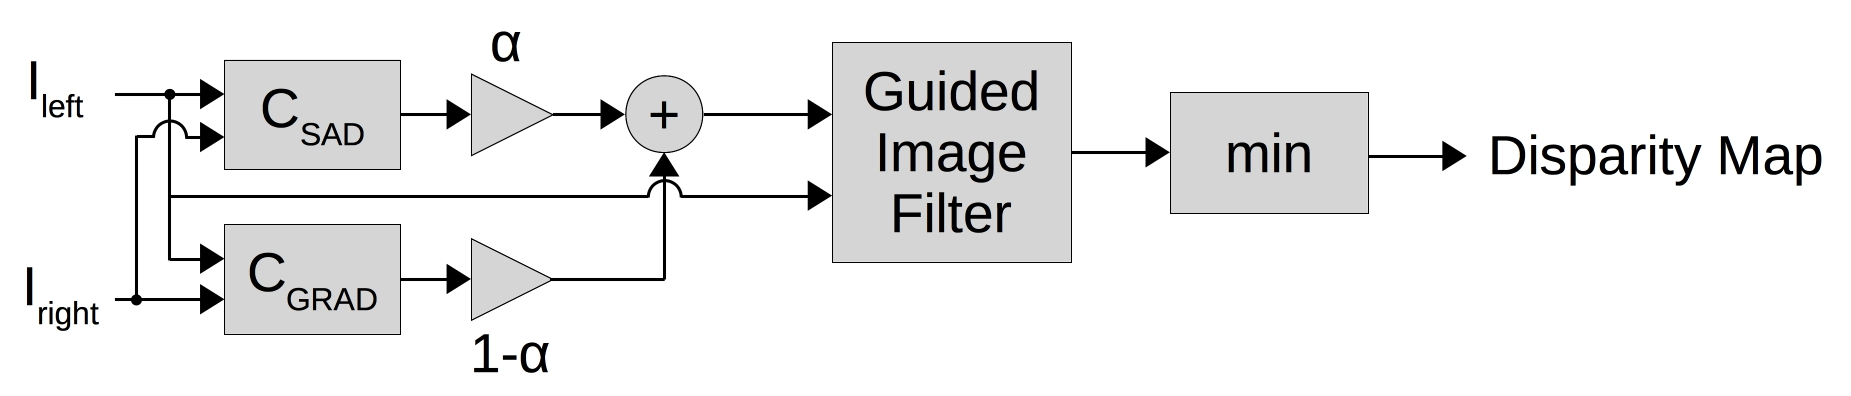
\includegraphics[scale=0.3]{figures/whole_system}
  \caption{Data flow graph of the whole system}
  \label{fig:whole_system}
\end{figure}

\begin{figure}[ht!]
  \centering
  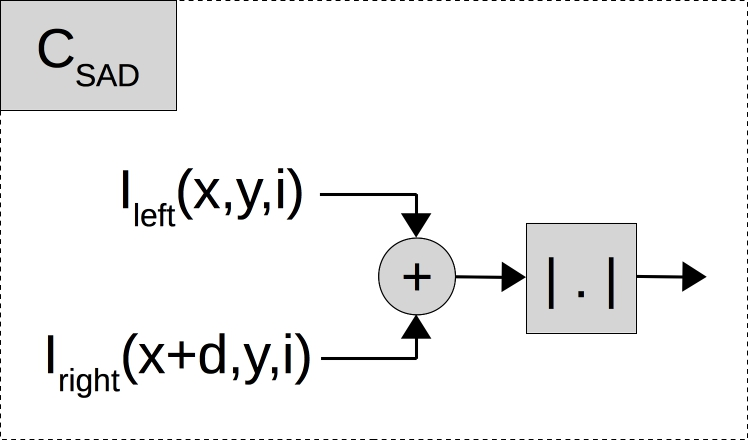
\includegraphics[scale=0.3]{figures/c_sad}
  \caption{Data flow graph of the $C_{SAD}$ block in figure \ref{fig:whole_system}}
  \label{fig:c_sad}
\end{figure}

\begin{figure}[ht!]
  \centering
  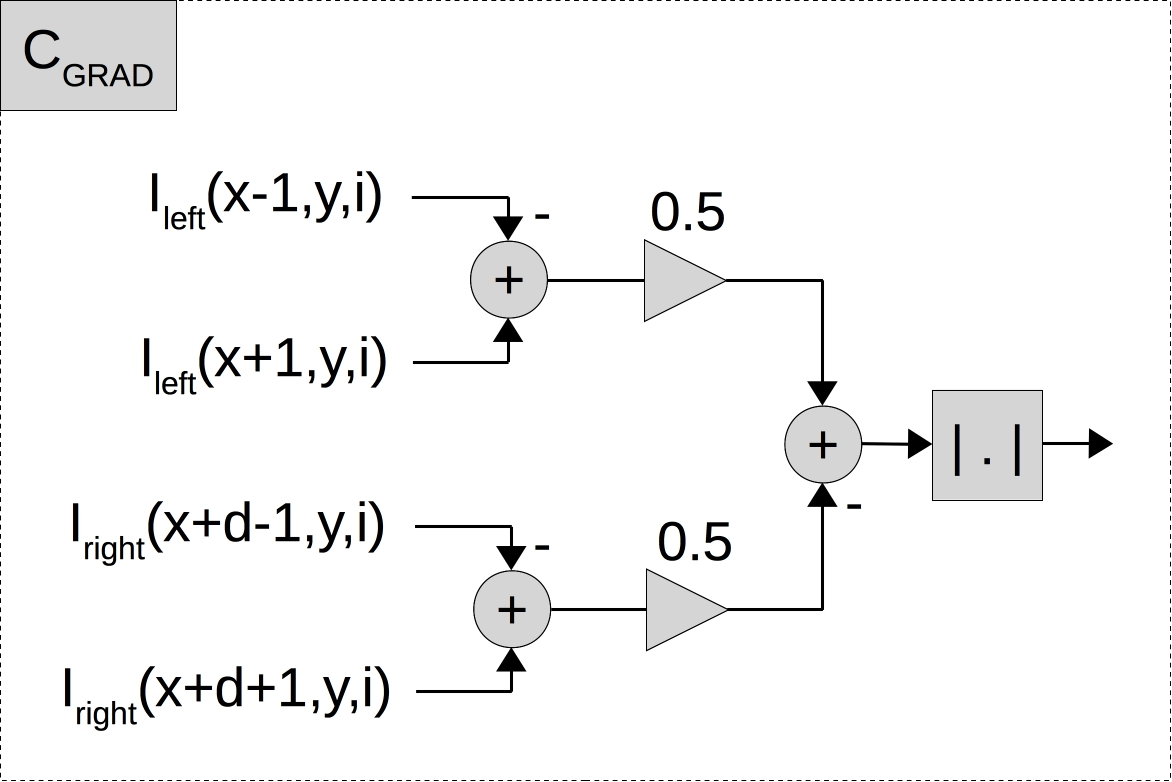
\includegraphics[scale=0.3]{figures/c_grad}
  \caption{$C_{GRAD}$ ikke sikker}
  \label{fig:c_grad}
\end{figure}

\begin{figure}[ht!]
  \centering
  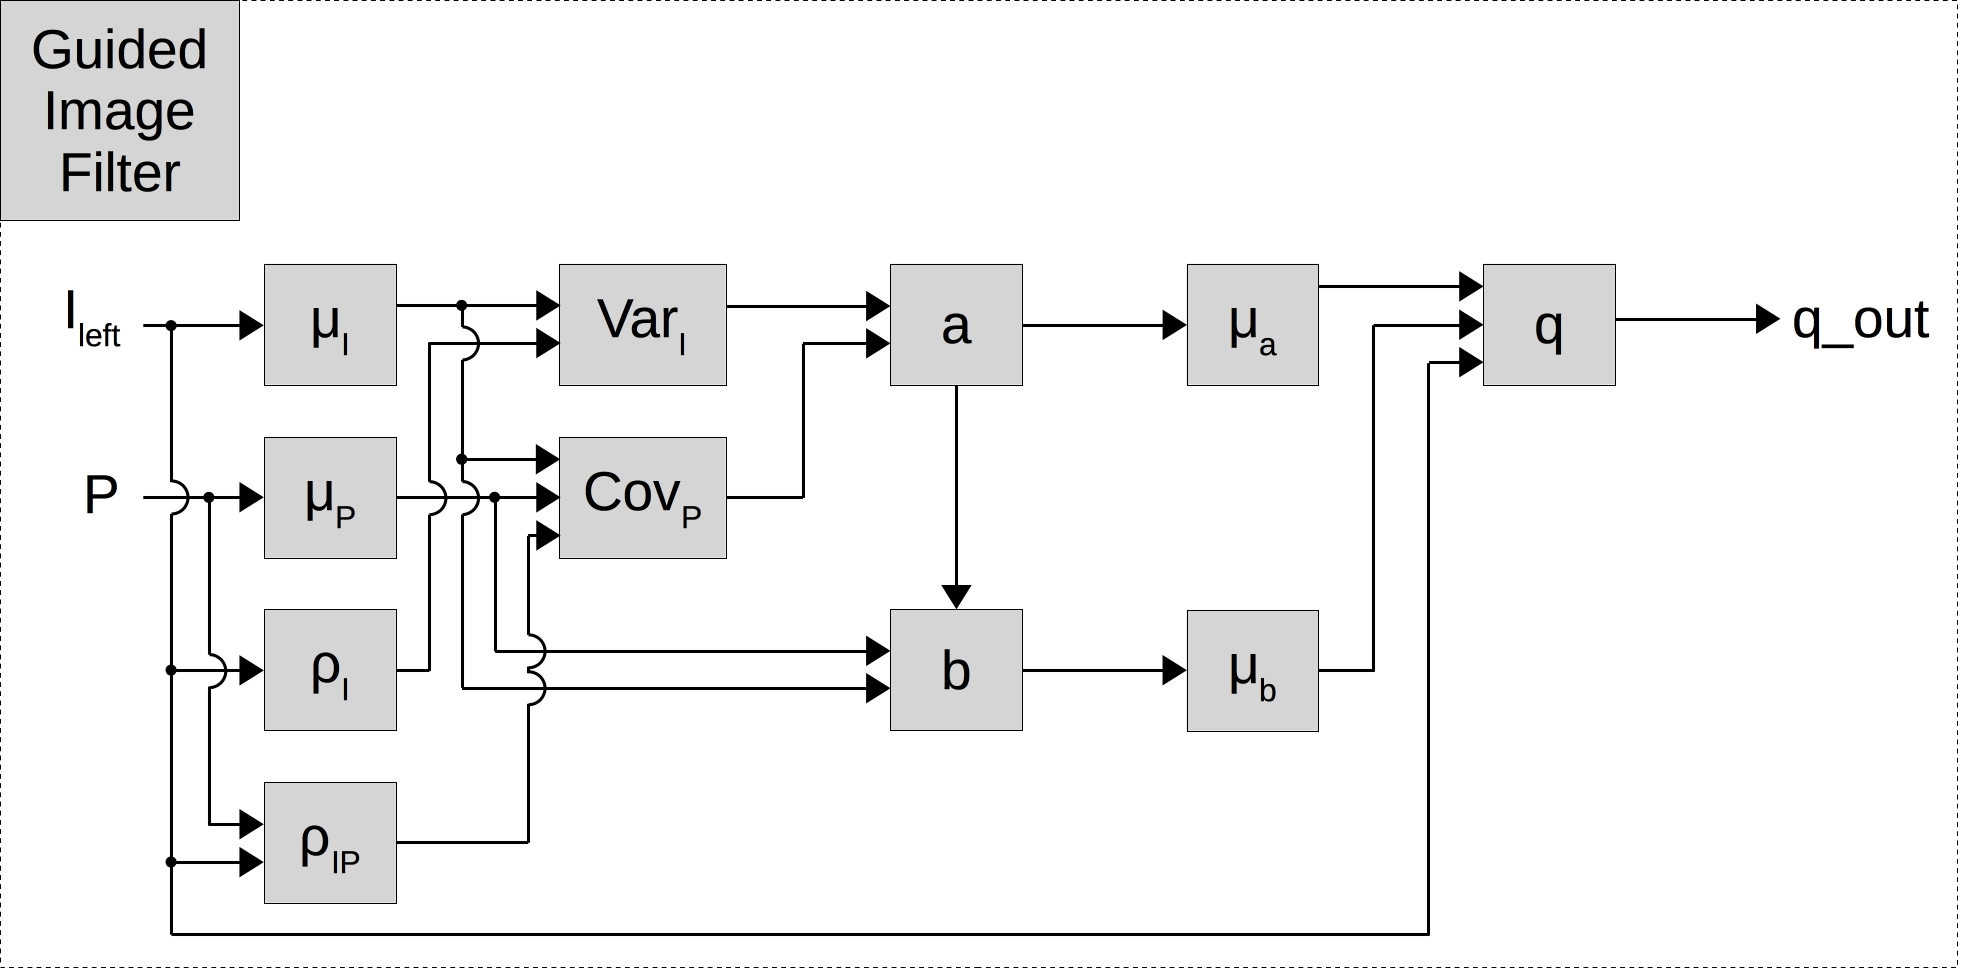
\includegraphics[scale=0.3]{figures/guided_image_filter}
  \caption{Guided image filter}
  \label{fig:Guided_image_filter}
\end{figure}

\begin{figure}[ht!]
  \centering
  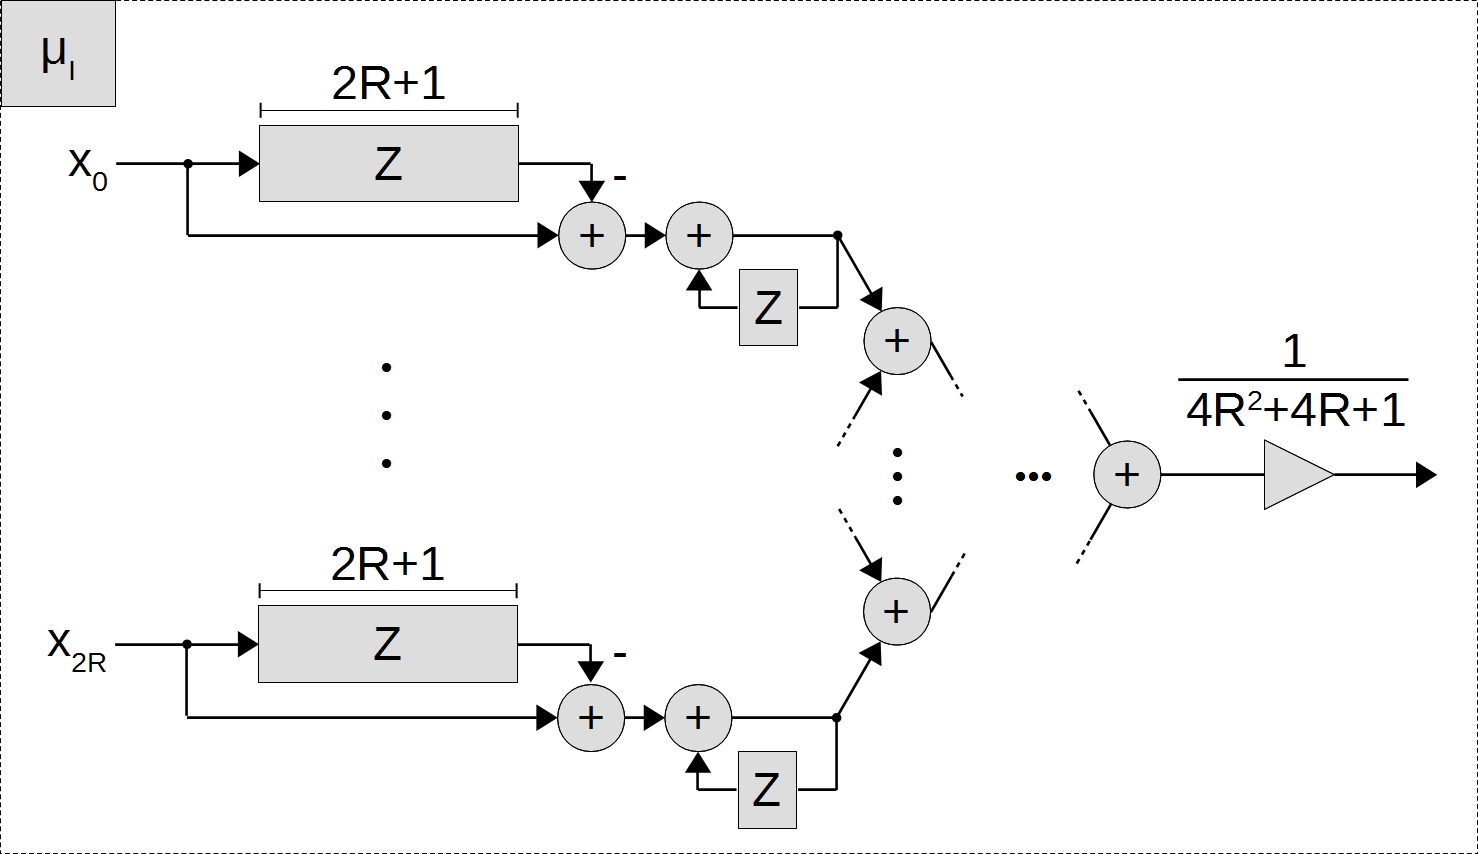
\includegraphics[scale=0.3]{figures/mean}
  \caption{Mean filter}
  \label{fig:mean}
\end{figure}

\begin{figure}[ht!]
  \centering
  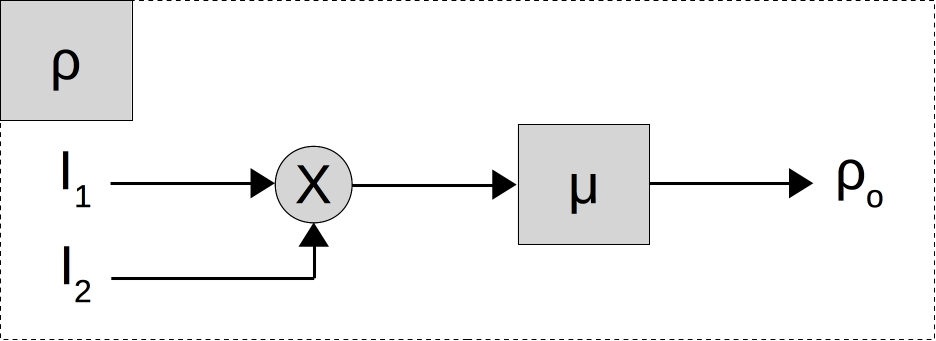
\includegraphics[scale=0.3]{figures/rho}
  \caption{Correlation}
  \label{fig:rho}
\end{figure}

\begin{figure}[ht!]
  \centering
  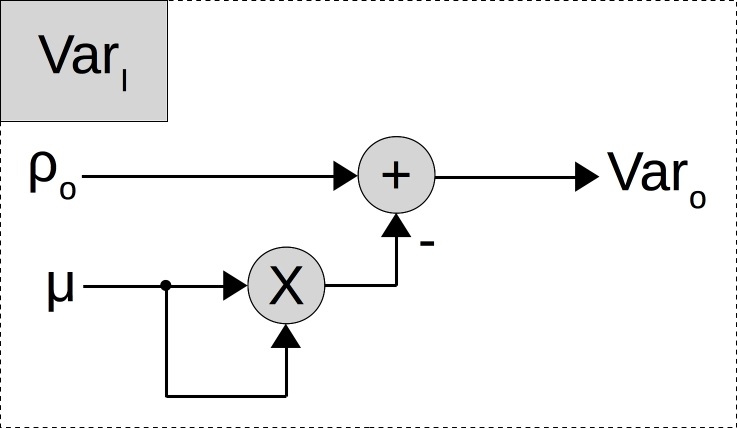
\includegraphics[scale=0.3]{figures/var_par}
  \caption{Variance}
  \label{fig:var_par}
\end{figure}

\begin{figure}[ht!]
  \centering
  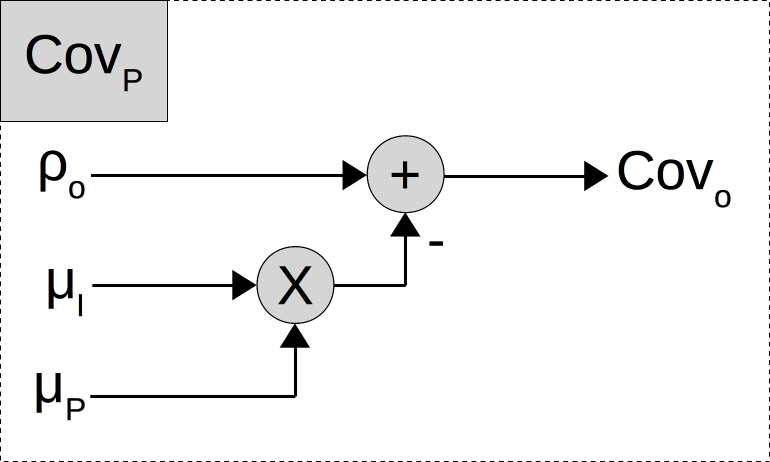
\includegraphics[scale=0.3]{figures/cov_par}
  \caption{Covariance}
  \label{fig:cov_par}
\end{figure}

\begin{figure}[ht!]
  \centering
  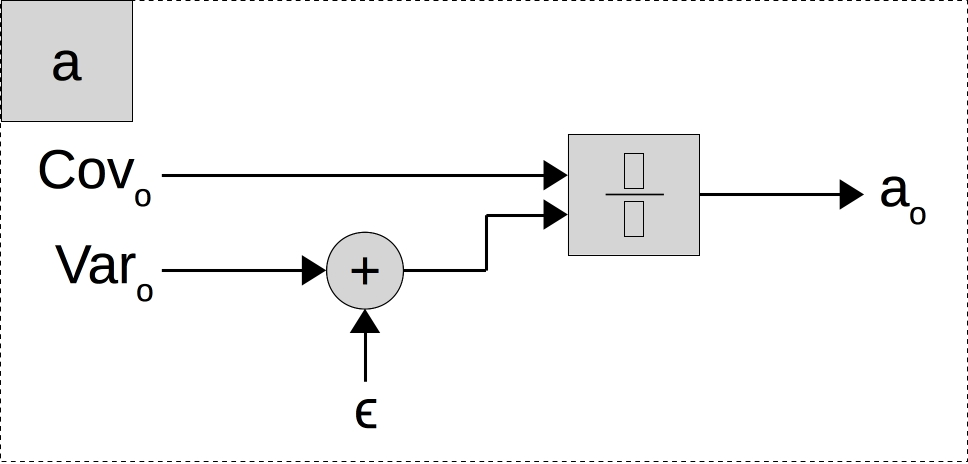
\includegraphics[scale=0.3]{figures/a_par}
  \caption{A box}
  \label{fig:a_par}
\end{figure}

\begin{figure}[ht!]
  \centering
  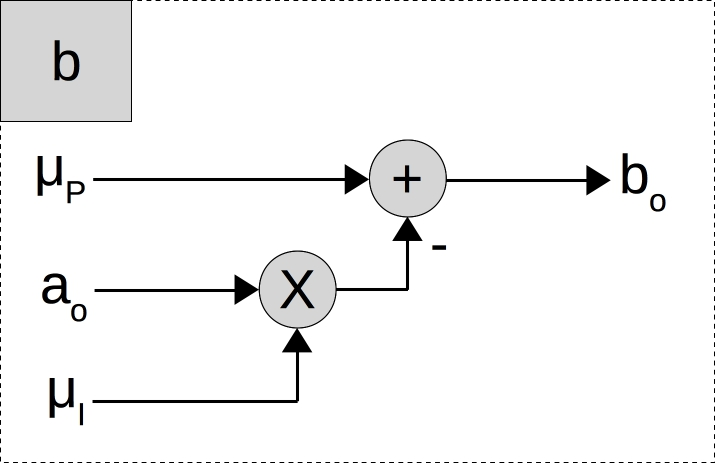
\includegraphics[scale=0.3]{figures/b_par}
  \caption{B box}
  \label{fig:b_par}
\end{figure}

\begin{figure}[ht!]
  \centering
  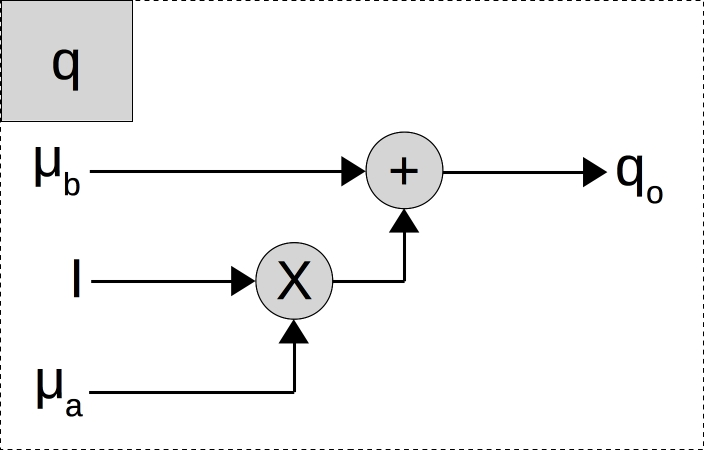
\includegraphics[scale=0.3]{figures/q_par}
  \caption{Q box}
  \label{fig:q_par}
\end{figure}

\color{gray}
\section*{noter til mig selv}
% ---------------------- udkommentere senere --------****
%lav dfg -> pg -> architecture. dette er steppet mellem algoritme og arkitektur domænerne i A3 modellen. Se første side i mm7 i reconf. kursuset. \\ 
%
%
%DSP ALG -> Precedence Graph -> Control data flow graph -> scheduling/allocation -> FSMD specification -> assignment -> architecture\\
%mm7 side (3) Force Directed Scheduling\\
%
%% links https://en.wikipedia.org/wiki/Analysis_of_parallel_algorithms
%Wanhammer \cite{wanhammer1999} side 244 i pdf / 229 i bogen:\\
%Precedence graphs. De beskriver in hvilken rækkefølge forskellige events (a,b,c) sker. order of occurrences of events\\
%Latency: dette er tiden tager at genere et output fra man har modtaget input.
%
%Throughput: dette er tiden mellem outputs
%
%Interleaving: increase throughput af sekventielle algoritmer.
%
%
%~\\
%Fra wiki: https://en.wikipedia.org/wiki/Analysis\_of\_parallel\_algorithms\\
%tag det med en gran salt. er nok hovedsagligt til General Purpose Processors (GPP)\\
%$p$ processors, $T_p$ time computation
%\begin{itemize}
% \item \textit{work}: total number of operations on the processors. Is equal to $T_1$.
% \item \textit{span}: the critical path. Length of longest series of data dependent operations. Is equal to $T_\infty$
% \item \textit{cost}: is $pT_p$ and describes the total time spent by all $p$ on both waiting and computing.
%\end{itemize}
%Laws:
%\begin{itemize}
%  \item \textit{Work law}: $pT_p \geq T_1$. the cost is at least equal to the work
%  \item \textit{Span law}: $T_p \geq T_\infty$. a finite number of processors, $p$, can't outperform an infinite number of processors
%\end{itemize}
%With these definitions and laws the following measures of performance can be given:
%\begin{itemize}
%  \item \textit{Speedup}: is the gain in speed when comparing parallel execution to sequential execution: $S_p = T_1 / T_2$
%  \item \textit{Efficiency}: is the speedup per processor: $S_p / p$
%  \item \textit{Parallelism}: is the ratio $T_1 / T_\infty$ and it describes the maximum speedup on any number of processors. By \textit{span law} the \textit{parallelism} bounds the speedup: if $p>T_1/ T_\infty$ then $T_1/T_p \leq T_1 / T_\infty < p$ 
%  \item \textit{Slackness}: is $T_1/(pT_\infty)$. a slackness than one implies (by span law) that perfect linear speedup is impossible on $p$ processors.
%\end{itemize}
%Execution on a limited number of processors\\
%Parallelitets analyse bliver normalt udført under den antagelse at man har et ubegrænset antal processor tilgængeligt. Dette er selvfølgelig ikke realistisk men ikke et problem da hvilken som helst beregning som kan laves på $N$ processorer kan også blive udført på $p$ processorer hvor $p < N$ ved at lade hver processor udføre flere "enheders" arbejde. \\
%Brent's law:\\
%$T_p \leq T_N + \dfrac{T_1 - T_N}{p}$ \\
%$T_p = O \left( T_N + \dfrac{T_1}{p} \right)$\\
%$\dfrac{T_1}{p} \leq T_p < \dfrac{T_1}{p} + T_\infty$ det viser at \textit{span} og \textit{work} giver nogle fornuftige grænser for computation time.\\
\color{black}

%\section{Optimization}

\section{VHDL + Simulation}

%\section*{Box filter / Mean function}
%\todo{this section should contain the design for my boxfilter or mean function}
%As seen from the guided image filter algorithm the mean function $f_{mean}(x)$ is used multiple q
%
%%\subsection*{Finite State Machine}
%\todo{beskriv FSM'en jeg har lavet (se figur 6.1) }
%\begin{figure}
%  \centering
%  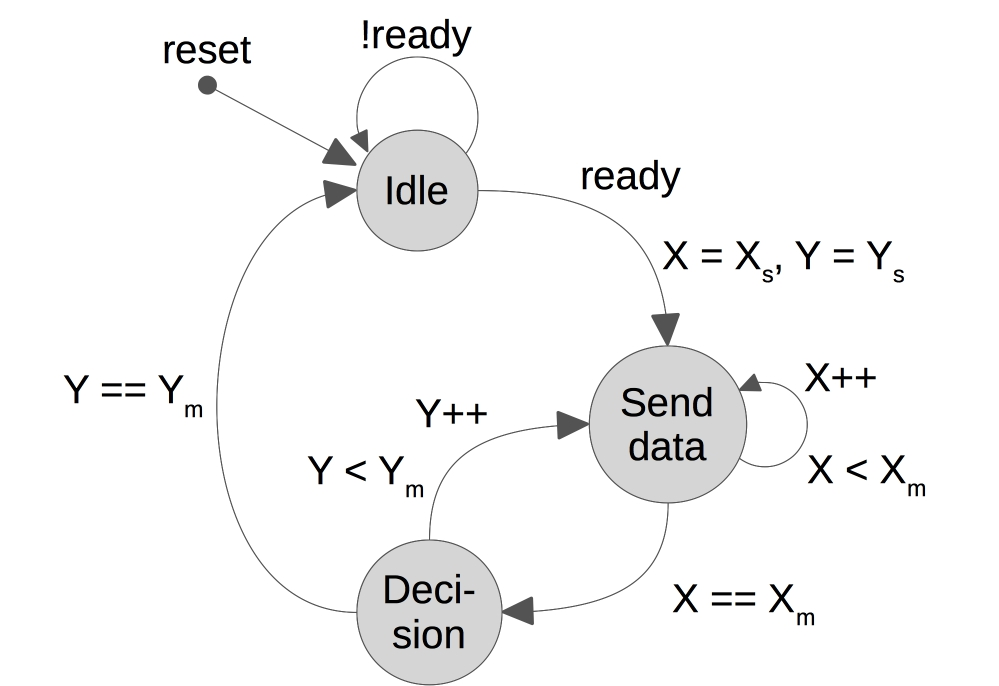
\includegraphics[width=0.5\textwidth]{figures/meanFSMv1.jpg}
%  \caption{TEXT GOES HERE}
%  \label{fig:LABEL}
%\end{figure}
%
%\subsection*{Memory}
%\begin{figure}
%  \centering
%  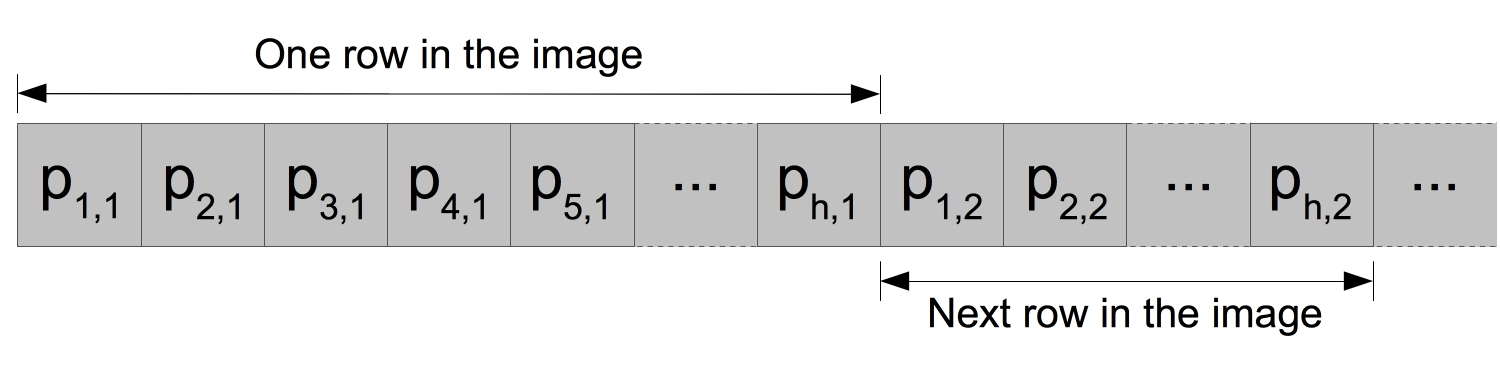
\includegraphics[width=0.5\textwidth]{figures/memdata.jpg}
%  \caption{TEXT GOES HERE}
%  \label{fig:LABEL}
%\end{figure}
%
%memory requirement: \\
%$3 \cdot 8$ bits per pixel (rgb image). test image is $741 \times 497$ so for the test image $8.838.648$ bits $\approx$ 9 megabit $\approx$ 1.1 megabyte.
%
%\subsection*{VHDL/Simulation}
%\todo{skriv om VHDL kode og simulation af filteret}
%
%\subsection*{Implementation/Test}
%\todo{skriv om implementation på FPGA'en og gerne verificere det virker}
%
